Implement fuzzy-cmeans from scratch

The paper this will be implemented from is titled, \textit{A Survey of Clustering Algorithms for Big Data: Taxonomy and Empirical Analysis}


From reference [1], the FCM algorithm is defined as follows: \newline

\begin{tcolorbox}
FCM pseudo-code:  \newline
Input: Given the dataset, set the desire number of clusters c, the fuzzy parameter m (a constant $> 1$), and the stopping condition, initialize the fuzzy partition matrix, and set stop = false.  \newline
Step 1. Do:  \newline
Step 2. Calculate the cluster centroids and the objective value J.\newline
Step 3. Compute the membership values stored in the matrix.  \newline
Step 4. If the value of J between consecutive iterations is less than the stopping condition, then stop = true.  \newline
Step 5. While (!stop)  \newline
Output: A list of c cluster centres and a partition matrix are produced.   
\end{tcolorbox}  


\begin{equation}
\label{eq:vk}
v_{k}=\frac{\sum_{i=1}^n{{\mu^{m}_{{i}{k}}{{\underline{p_{i}}}}}}}{\sum_{i=1}^n{{\mu^{m}_{{i}{k}}}}}
\end{equation}
   
\begin{equation}
\label{eq:distance}     
{\vert{\underline{p_{i}}}-{\underline{v_{k}}}\vert}=\sqrt{\sum_{i=1}^{n}{({\underline{x_{i}}}-{\underline{v_{k}}})^2}}
\end{equation}
  
\begin{equation}
\label{eq:objective_function}
J=\sum_{i=1}^{n}{\sum_{k=1}^{c}{\mu^{m}_{{i}{k}}{\vert{\underline{p_{i}}}-{\underline{v_{k}}}\vert^{2}}}}
\end{equation}  

\begin{equation}
\label{eq:membership_value}
{\mu^{m}_{{i}{k}}}=\frac{1}{\sum_{l=1}^{c}{(\frac{{\vert{\underline{p_{i}}}-{\underline{v_{k}}}\vert^{2}}}{{\vert{\underline{p_{i}}}-{\underline{v_{l}}}\vert^{2}}})}^{\frac{2}{m-1}}}
\end{equation}
An example of two handwriting samples is shown as images in figure~\ref{fig:image1} and figure~\ref{fig:image2}. These images were produced using the imshow function from the matplotlib python library.\newline

\begin{center}
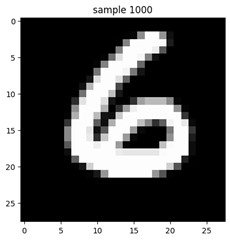
\includegraphics[width=0.35\textwidth]{image1.png}
\captionof{figure}{Handwriting Sample 1000\label{fig:image1}}
\end{center}

\begin{center}
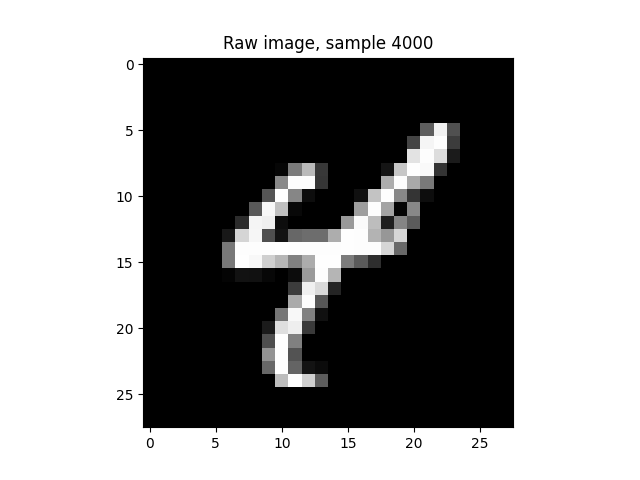
\includegraphics[width=0.35\textwidth]{image2.png}
\captionof{figure}{Handwriting Sample 4000\label{fig:image2}}
\end{center}    
        